\documentclass[12pt]{article}  
\usepackage{latexsym,graphicx}
\usepackage{amssymb}
\usepackage{tikz}
\usetikzlibrary{positioning,shapes.gates.logic.US}
\voffset=-.8cm
\hoffset=-1.5cm
\setlength{\textheight}{23cm}
\setlength{\textwidth}{16cm}
\pagestyle{myheadings}
\newtheorem{q} {Q}
\newcommand{\beq}{\begin{q}\hskip.01cm)\hskip.03cm}
\newcommand{\eeq}{\end{q}\newpage}
\newcommand{\df}{\displaystyle\frac}
\newcommand{\dar}{\downarrow}
\newcommand{\ra}{\rightarrow}
\newcommand{\lra}{\leftrightarrow}
\markright {Dr. Petrescu CCP MATH163 Practice Exam 1}
\begin{document}
{\bf Practice Exam 1 Discrete Mathematics 1 } \vskip0.2cm
\vskip.1cm{\bf This is a mandatory homework. Show all your work to get credit. }  \vskip0.2cm 
{\bf Name}: Ayush Pandejee {\bf Due Date}: {\underline{10/06/23}} \vskip.5cm
%%questions   \eeq

\beq The following sign is at the entrance of a restaurant: ``No shoes, no shirt, no service." Write this sentence as a conditional proposition. \\

-Lets set p equal to shoes, q equal to shirt, and r equal to service. If p equals shoes, $¬\lnot p$ equals no shoes. Using this logic, we can come to the solution that ($¬\lnot p \lor ¬\lnot q) \ra ¬\lnot r$.
\eeq

\beq Write these system specifications in symbols using the propositions:\\v: ``The user enters a valid password,"\\a: ``Access is granted to the user,"\\c: ``The user has contacted the network administrator,"\\and logical connectives. Then determine if the system specifications are consistent (i.e. all 3 statements can be simultaneously true).\\(i) ``The user has contacted the network administrator, but does not enter a valid password."\\(ii) ``Access is granted whenever the user has contacted the network administrator or enters a valid password."\\(iii) ``Access is denied if the user has not entered a valid password or has not contacted the network administrator." \\

i) C $\land$ $\lnot V$\\

ii) ($C \lor V$) $\ra$ A\\

iii) ($\lnot V \lor \lnot C$) $\ra$ $\lnot A$\\

Lets set the truth values for V, A, and C as True, True, and False respectively.\\

C $\land$ $\lnot V \equiv False \land True = False$\\

($C \lor V$) $\ra A \equiv (False \lor True) \ra True = True \ra True = True$\\

($\lnot V \lor \lnot C$) $\ra$ $\lnot A \equiv (False \lor True) \ra False = True \ra False = False$\\

Since all of the three statements don't have the same truth value in the end, they are not consistent.
\eeq

\beq Solve this puzzle: You meet two people, A and B. Each person either always tells the truth or always lies. Person A tells you, ``We are not both truthtellers.''\\Determine, if possible, which type of person each one is. \\

So we know that there are two people. One always tells the truth and the other always lies. A says that we not both truthtellers. Lets say A was telling a lie. That would not make sense because if he was a liar, then why would he tell you the truth this time. If A was a truthteller, than it would make sense because because he is telling the truth about both of them not being a truthteller. That means B is a liar and A is telling the truth. \\
\eeq

\beq Here is a newspaper headline:\\``Legislature Fails to Override Governor's Veto of Bill to Cancel Sales Tax Reform." \\Did the legislature vote in favor of or against sales tax reform?\\

Legislature voted in favor for the sales tax reform. The statement says that Legislature fails to override, which means the wanted to override the veto bill. The veto bill was in response to cancel sales tax reform. If the Governer vetoed that bill to cancel it, and the legislature wants to override it, that means they want the sales tax reform.
\eeq

\beq Prove that  $  p  \rightarrow  (q \lor r ) \equiv  (p\land \lnot q)  \rightarrow  r $ by using a series of logical equivalences.\\

First, we know that $(p\land \lnot q)  \rightarrow  r \equiv (p \ra r) \lor (\lnot q \ra r)$. We also know that $(p \ra r) \lor (\lnot q \ra r) \equiv (\lnot p \lor r) \lor ( q \lor r)$. This is also equivalent to $\lnot p \lor (r \lor r \lor q)$ due to association. Next, $\lnot p \lor (r \lor r \lor q) \equiv \lnot p \lor (q \lor r)$. Finally, $\lnot p \lor (q \lor r) \equiv p  \ra  (q \lor r)$. This proves that the two expressions are equivalent.
\eeq

\beq Consider this sentence, which is Section 2 of Article I of the U. S. Constitution: \\``No person shall be a Representative who shall not have attained the age of twenty-five years, and been seven years a citizen of the United States, and who shall not, when elected, be an inhabitant of that state in which he shall be chosen."\\(a) Rewrite the sentence in English in the form ``If . . . , then . . . ". \\(b) Using the predicates A(x): ``x is at least twenty-five years old," C(x): ``x has been a citizen of the United States for at least seven years," I(x): ``x, when elected, is an inhabitant of the state in which he is chosen," and R(x): ``x can be a Representative," where the universe for x in all four predicates consists of all people, rewrite the sentence using quantifiers and these predicates. [Note: At the time at which the U. S. Constitution was ratified, the universe for x consisted of landowning males.]\\

a) If you are a Representative, then you are atleast 25 years old, been a citizen of the United States for atleast 7 years, and an inhabitant of the state from which you are chosen.\\

b) $\forall x$ $|$ (A(x) $\land$ C(x) $\land$ I(x)) $\ra$ R(x)
\eeq

\beq Suppose that the universe for x and y is \{1,2,3\}. Also, assume that P(x,y) is a predicate that is true in the following cases, and false otherwise: P(1,3),P(2,1),P(2,2),P(3,1),P(3,2),P(3,3). Determine whether each of the following is true or false:\\(a) $\forall    y\exists    x (x\neq y \wedge P (x, y))$.\\(b) $\forall    x\exists    y (x\neq y \wedge \neg P (x, y))$.\\(c) $\forall    y\exists    x (x\neq y \wedge \neg P (x, y))$.\\

a) A states that for every Y value of the 9 possible combinations, there exists a X value which fulfils the statement from the 6 given cases that are true. If we go through all of the Y values, we can see from the possible true cases that there exists an X value for every Y value which fulfils this statement. So A is true. \\

b) B states that for every X value, there exists a Y value from the 6 true cases that makes the $\lnot P(x,y)$ true. This is not true because we can see from the possible true cases that there exists an Y that makes P(x,y) true. So this makes B false.\\

c) C states that for every Y value, there exists a X value from the 6 true cases that makes the $\lnot P(x,y)$ true. This is also not true because we can see from the possible true cases that there exists an X that makes P(x,y) true. So this makes C false aswell.
\eeq

\beq Determine whether this argument is valid: \\Lynn works part time or full time.\\ If Lynn does not play on the team, then she does not work part time. \\If Lynn plays on the team, she is busy.\\Lynn does not work full time.\\Therefore, Lynn is busy. \\

The argument is valid. We can first start with the fourth sentence. It says that Lynn does not work full time. If we take this and bring it back to the first statement, it means that Lynn works only part time because the fourth statement states that Lynn does not work full time. Now, the second statement states that if Lynn does not play, she does not work part time. This means that if she works part time, she plays on the team (contrapositive). Now, we can go to the third statement which states that if she plays on the team, she is busy. This brings us to the last statement, which makes the entire series true.
\eeq

\beq   Give a proof by contradiction of: ``If n is an even integer, then $3n + 7$ is odd."\\

By using a proof by contradiction, we have to assume the opposite case of the statement, which gives us "If n is an even integer, then 3n + 7 is even." Let n = 2k (2 times any integer, k, gives us an even value). Plugging in 2k, we get 6k + 7. 6k + 7 also equals 2(3k + 3) + 1. We can set 3k + 3 equal to m. This gives us 2m + 1. This means that no matter what the integer is, 3n + 7 cannot be even because 2m + 1 is not even. So this means that 3n + 7 is odd. 
\eeq

\beq Find the output of the following logic gate:\vskip.8cm 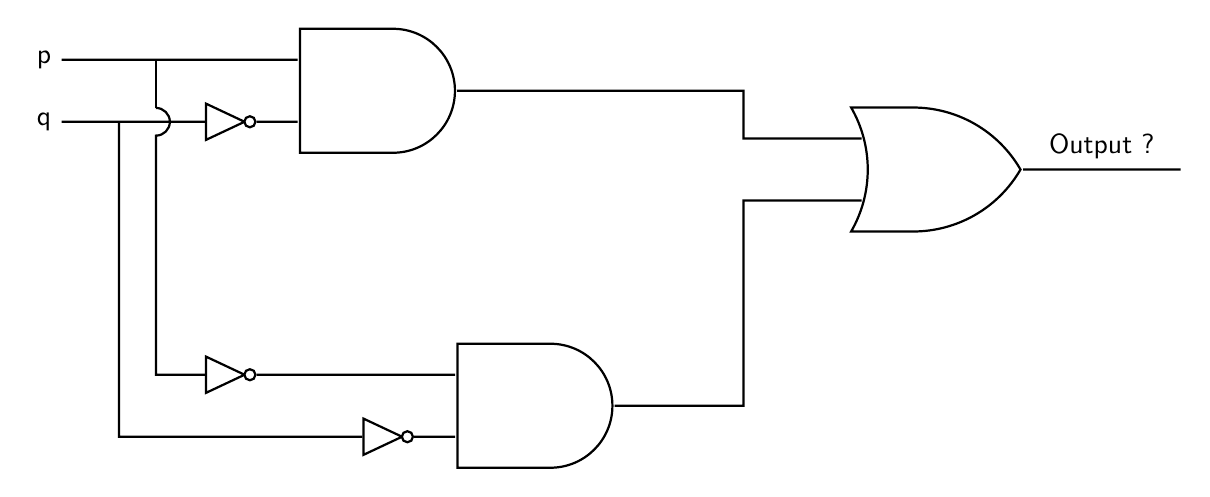
\begin{tikzpicture}[
% you can find documentation here: https://tikz.dev/library-circuits#autosec-5292
        %Environment config
        font=\sffamily,
        thick,
        %Environment styles
        GateCfg/.style={
            logic gate inputs={normal,normal,normal},
            draw,
            scale=2
        }
    ]
    \path
        (0,0) node[and gate US,GateCfg](AND1){} 
            ++ (2,-4) node[and gate US,GateCfg](AND2){} 
            ++ (5,3) node[or gate US,GateCfg](OR1){}
        (AND1.input 3)
            ++ (-1,0) node[not gate US, draw](N1){}
        (AND2.input 3)
            ++ (-1,0) node[not gate US, draw](N2){}
        (AND2.input 1 -| N1)
            node[not gate US, draw](N3){};

    \draw
        (OR1.input 1) -- ++(-1.5,0) |- (AND1.output)
        (OR1.input 3) -- ++(-1.5,0) |- (AND2.output)
        (N2.output)--(AND2.input 3)
        (N1.output)--(AND1.input 3)
        (N3.output)--(AND2.input 1)
        (AND1.input 1) 
            -- ++(-3,0) coordinate (init) node[anchor=east]{p}
            node[pos=0.6](temp){}
        (N1-| temp)
            ++(0,5pt) edge (temp.center)
            arc (90:-90:5pt) |- (N3.input)
        (init |- N1) node[anchor=east]{q} 
            -- (N1.input) node[pos=0.4](temp2){}
        (temp2.center) |- (N2.input)
        (OR1.output) -- ++(2,0) node [midway,anchor=south]{Output ?};
    \end{tikzpicture}\\ 

($p \land \lnot q) \lor (\lnot p \land \lnot q$)
  \eeq

  \beq  Prove, using whatever method you want, that at least one of the real numbers $a_1, a_2, ..., a_n$ is greater than or equal to the average of these numbers.\\
  
  We can prove this by contradiction. This means that we have to prove that one of the real numbers $a_1, a_2, ..., a_n$ is less than the average of the numbers. To get the average of the numbers, you have to do $(a_1 + a_2 + ...+ a_n)/n$. Since we are proving by condtradiction, that means that an individual value, $a_i$ is less than $(a_1 + a_2 + ... + a_n)/n$. We can add up the sum of all of the individual values, $(a_1 + a_2 + ... + a_n)$, and set it less than $n*(a_1 + a_2 + ... + a_n)/n$. The reason why we do this is because since $a_i$ is a singular, individual value, we also have to account for all of the other individual values so we can add all of them up and set it less than the average times n. This gives us $(a_1 + a_2 + ... + a_n) < n*(a_1 + a_2 + ... + a_n)/n$. If we simplify the right side, we get $(a_1 + a_2 + ... + a_n) < (a_1 + a_2 + ... + a_n)$, which cannot be true. So, since one of the real numbers $a_1, a_2, ..., a_n$ cannot be less than the average of these numbers, it must be greater than or equal to the average of the numbers, which proves the original statement. 
  \eeq

  \beq Prove by contraposition: $x\in {\mathbb R}, x^2 - 6x+5>0 \rightarrow x\geq 5\;  \lor \; x\leq 1$\\
  
  By using proof by contraposition, we have to prove that $x < 5\; \land\; x > 1$ $\ra$ $x^2 - 6x+5 \leq 0$. We can start off by factoring the equation $x^2 - 6x+5$ which gives us $(x - 5)(x - 1)$. If x is both less than 5 and greater than 1, that means that no matter the x value, it will always be less than or equal to zero. It will always be less than or equal to zero because since x is less than 5, anything less than 5 plugged into x - 5 gives us a negative number. Any negative number multiplied by a positive gives you a negative value which is less than zero. This proves the contraposition to be true, which makes the original statement true as well.
  \eeq
  
  \beq Prove by cases: $ x  y \in {\mathbb R}, y \neq 0 \rightarrow \df{|x|}{|y|} = |\df{x}{y}|$
  
  Case 1: x = 0, y\\

  $\df{|0|}{|y|} = |\df{0}{y}|$\\
  
  This makes case 1 true because regardless of the y value, both of these are equal to each other.\\

  Case 2: $x > 0, y > 0$\\

  This means that both x and y are positive, so $|x| = x$ and $|y| = y$. This means that $\df{|x|}{|y|} = |\df{x}{y}|$ because $\df{x}{y} = \df{x}{y}$. So case 2 is also true.\\

  Case 3: $x < 0, y < 0$\\

  For $\df{|x|}{|y|}$, we know that $|-x| = x$ and $|-y| = y$. So $\df{|-x|}{|-y|} = \df{x}{y}$. We also know that $|\df{-x}{-y}| =  \df{x}{y}$. This makes both of them equivalent and case 3 true as well.\\

  Case 4: $x > 0, y < 0$\\

  For $\df{|x|}{|y|}$, we know $|x| = x$ and $|-y| = y$. Using this, $\df{|x|}{|-y|} = \df{x}{y}$, and $|\df{x}{-y}| =  \df{x}{y}$. This makes case 4 true as well.\\

  Case 5: $x < 0, y > 0$\\

  We know that $|-x| = x$ and $|y| = y$. Using this, $\df{|-x|}{|y|} = \df{x}{y}$, and $|\df{-x}{y}| =  \df{x}{y}$. This makes case 5 true as well.\\

  These 5 cases prove the original statement since all of them are true.
  \eeq

%%questions
\end{document}